\subsection{Attention mechanism}
\label{appendix:attention}

Most of the attention mechanisms are introduced in the transformer paper \cite{transformer}.

The cross-attention mechanism is explained partly in section \ref{subsec:cross_attention}. Here we dive deeper into the attention mechanism and explore the building blocks of transformers and other blocks used in image and video synthesis models.


\subsubsection{Self-attention}

Self-attention allows us to model the weight of different parts of an input sequence. In short, it gives us indication on how much focus to give to different elements in a sequence, which considers realtionships between then.

An application example of self-attention is in Stable Diffusion (section \ref{sec:stable_diffusion}) where self-attention is used between patches of an image to model the relationships between, similar to how convolution models the local relationships of pixels, but in self-attention we model global relationships.

The \textbf{input} to the self-attention block is a sequence (vector) $X \in \mathbb{R}^{n \times d}$ and the \textbf{output} has the same dimension.

Then we apply linear projections: $Q = XW_Q$, $K = XW_K$, $V = XW_V$ where $W_Q, W_K, W_V \in \mathbb{R}^{d \times d}$ are learnable projection matrices (basically they are weight matrices that are learned during training and are assigned random value initially).

We can think of \textbf{Q}(uery), \textbf{K}(ey), \textbf{V}(alue) as text search in Google. When we query Google, we get keys as a result (list of pages), which is not what we are looking for. When we click on a page, then we get the value. Therefor Google has to find \textbf{similarity} between query and the keys.

We can think of similarity in linear algebra as \textbf{cosine similarity} between matrices: $\text{CosSim} = \frac{A \cdot B}{||A|| ||B||}$.

The self-attention mechanism is defined as:

\begin{equation*}
    \text{Attention}(Q, K, V) = \text{softmax}\left( \frac{QK^T}{\sqrt{d_k}} \right) V
\end{equation*}

where $d_k$ is the dimension of the key vector, $\sqrt{d_k}$ normalizes the large magnitude of the dot product (which stabilizes the gradients and the training), and we apply softmax to the attention weights (which converts the vector to a probability distribution between 0 and 1, which gives probability to tokens in the sequence). We then multiply (dot product) the attention weights with the value matrix to get the output. $K$ is transposed to match the dimensions of $Q$ (so we can multiply them).

\begin{lstlisting}[language=Python, breaklines=true, caption={Full implementation of a single self-attention block.}]
class SelfAttention(nn.Module):
"""
embed_dim (int): The dimensionality of the input embeddings.
attention_dim (int): The dimensionality of the attention space / attention vectors (Q, K, V).
"""
def __init__(self, embed_dim, attention_dim):
    super(SelfAttention, self).__init__()
    # Linear projections for Q, K, V
    self.W_Q = nn.Linear(embed_dim, attention_dim)
    self.W_K = nn.Linear(embed_dim, attention_dim)
    self.W_V = nn.Linear(embed_dim, attention_dim)
    self.scale = torch.sqrt(torch.tensor(attention_dim, dtype=torch.float32))

def forward(self, X):
    Q = self.W_Q(X)
    K = self.W_K(X)
    V = self.W_V(X)

    attention_scores = torch.matmul(Q, K.transpose(-2, -1)) / self.scale
    attention_weights = F.softmax(attention_scores, dim=-1)
    attention_output = torch.matmul(attention_weights, V)

    return attention_output
\end{lstlisting}










\subsubsection{Multi-head attention}

The input matrices (Q,K,V) derive from the same input sequence. In comparison, in cross-attention, we relate two different sequences. Cross-attention is particularly useful in tasks that requires alignment between different sequences, like in translation tasks, whereas in self-attention and multi-head attention we are looking for relationships within the same sequence, like in sentiment analysis.

Multi-head attention is a concatenation of multiple self-attention heads, each with its own set of weights $W_i^Q$, $W_i^K$, $W_i^V$. That means that each attention head can learn different relationships between the same elements in the same sequence. After concatenation we apply dot product with the output weights matrix $W^O$:

\begin{equation}
    \begin{aligned}
        \text{head}_i = \text{Attention}(QW_i^Q, KW_i^K, VW_i^V)  \\
        \text{MultiHead}(Q, K, V) = \text{Concat}(\text{head}_1, ..., \text{head}_h)W^O
    \end{aligned}
\end{equation}









\subsubsection{Cross-attention}

Cross-attention is used to relate two different sequences, between the query and the key-value pairs. The query sequence is used to get the attention weights, which are then applied to the key-value pairs. This is useful in tasks that require alignment between different sequences, like in translation tasks.

In cross-attention we first project the input $X$ onto the $Q$ matrix. And in the case of Stable Diffusion (section \ref{sec:stable_diffusion}), we project the text embeddings (or other conditional signal) onto the $Q$ and $V$ matrices. This way the latent vector is conditioned on text. Thats the main difference between self-attention and cross-attention.

Projection is done like so: $Q = XW_Q$, $K = YW_K$, $V = YW_V$ where $X$ is the input sequence, $Y$ is the sequence we want to relate to, and $W_Q, W_K, W_V \in \mathbb{R}^{d \times d}$ are learnable projection matrices.

Cross-attention is often implemented in multi-head fashion, therefor we can use the same implementation as in multi-head attention.

Because the math is the same, just with different notation, cross-attention is the same as self-attention but with different input sequences.







\subsubsection{Axial attention}

Axial attention \cite{axial_attention}, as described in VideoGPT \cite{videogpt}, is a variant of the self-attention block. One of the biggest problem of self-attention is the quadratic complexity: particularly in Image-GPT, where the entire image is self-attended. One of the solutions is the axial attention. Where as in typical self-attention the complexity is $O(n^2)$, in axial attention the complexity is $O(n\sqrt{n})$ (where $n$ is the width/height of the image).

\begin{figure}
    \centering
    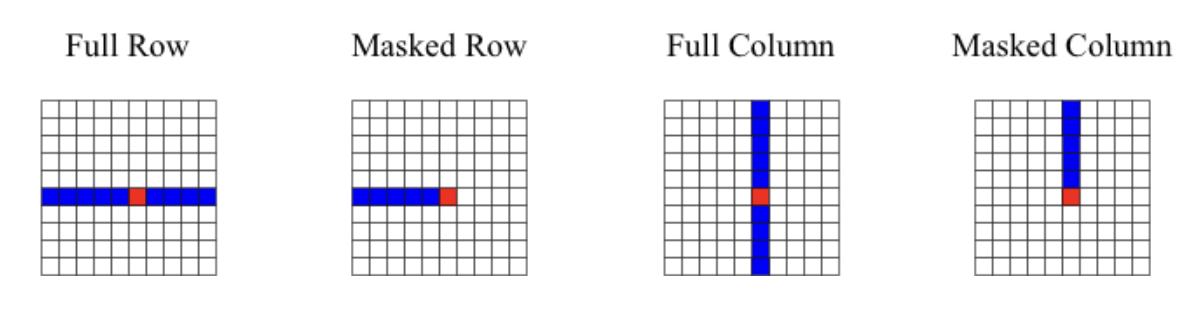
\includegraphics[width=0.75\textwidth]{images/appendix/attention/axial.png}
    \caption{Types of axial attention layers which are the building blocks of axial transformer.}
    \label{fig:axial_attention}
\end{figure}

Axial attention first attends to the masked column and then masked row, instead of the full input sequence (we only focus on one axis at a time instead of all of the pixels). When we roll the 2D image into 1D image, we typically go from top-left to bottom-right, in that order. So the masked row, column intend to save computations. This masking can be seen in figure \ref{fig:axial_attention}. Why the row, column are masked? Because of the order of pixels that are flattened to 1D tensor, we go from top-left to bottom-right and as autoregressive pixel prediction model, the model will be predicting the pixel $p_{i, j}$ and not $p_{i+1, j}$ or $p_{i, j+1}$. It only depends on previous pixels.

Although axial transformer is not attending to every pixel for every prediction, it still captures spatial global context.


